% PVLDB Volume 20, Scalable Data Science category (8 pages excluding references).
% Companion to paper/pvldb1t (Experiment, Analysis & Benchmark), under submission together.
% Build: pdflatex main; bibtex main; pdflatex main; pdflatex main
% Figure data is read from ../pvldb1t/figdata (produced by fig_data.py from the record logs).
\documentclass[sigconf, nonacm]{acmart}
%%% VLDB block start %%%
\usepackage{pvldb}
%%% VLDB block end %%%
\renewcommand\vldbdoi{XX.XX/XXX.XX}
\renewcommand\vldbpages{XXX-XXX}
\renewcommand\vldbavailabilityurl{https://github.com/ahb-sjsu/turboquant-pro/tree/master/benchmarks/fleet}

\usepackage{booktabs}
\usepackage{pgfplots}
\pgfplotsset{compat=1.18}
\usepgfplotslibrary{statistics}
\usetikzlibrary{arrows.meta,positioning,calc,fit,backgrounds}
\setlength{\emergencystretch}{1.5em}

\begin{document}
\title{A Trillion Vectors in the Smallest Job Class [Scalable Data Science]}
\subtitle{Building and measuring a sharded vector index on a shared research cluster with one CPU and two gigabytes per job}

\author{Andrew H. Bond}
\orcid{0009-0003-2599-6158}
\affiliation{%
  \institution{San Jos\'e State University}
  \city{San Jos\'e}
  \state{California}
  \country{USA}
}
\email{andrew.bond@sjsu.edu}

\begin{abstract}
A sharded vector index of one trillion 4-bit quantized rows, 24 TB on 500 block volumes, was built
and then measured exactly on the National Research Platform, a Kubernetes cluster shared by many
research groups, with no reserved capacity. Every job in the build and the measurement requested
one CPU and two gigabytes of memory, the smallest class the cluster offers. Three design choices
made that possible. The corpus is defined by a seed and regenerated where it is needed, so the
build moved no corpus bytes and a lost volume was rebuilt from its seed in under four hours. Every
job is idempotent on its volume, so a failed or duplicated job costs a retry and never a wrong
result. A pool of per-server jobs, submitted through a controller that yields when the cluster is
busy, recovers from failures by a small number of explicit rules rather than by operator
attention. The build of 500 servers took seven weeks of background capacity, and the exact scan
and five routed passes over the whole index took four days, 1349 CPU-hours, 1502 submissions and
1350 completions, with six pods replaced by hand. The recall this measured is reported in a
companion paper. Here we describe the index layout, the corpus generator, the job shape, the pool
and its rules, what failed and how often, and what the whole run cost.
\end{abstract}

\maketitle

%%% do not modify the following VLDB block %%
%%% VLDB block start %%%
\vldbtopmatter
%%% VLDB block end %%%

\section{Introduction}

Measuring a vector index at a trillion rows needs a trillion rows in one place and an exact scan of
all of them. Few groups own that much capacity. Research clusters that federate many sites have it
in aggregate, but they share it, reserve nothing for any one user, and expect jobs that come and go
without supervision. This paper describes how a trillion-row index was built and scanned exactly on
such a cluster, the National Research Platform's Nautilus \cite{weitzel2025nrp}, with every job in
the smallest resource class the platform offers.

The run exists to answer a measurement question, whether routed search over a sharded index loses
anything the exact scan finds as the index grows to $10^{12}$ rows. The companion paper
\cite{bond2026recall} reports that answer. This paper is about the machinery. It makes three
points. A corpus defined by a seed turns a 24 TB build into computation with no data movement and
turns the loss of a volume into a rebuild. A scan over memory-mapped shards fits one CPU and two
gigabytes once three choices are made about queries, open shards and block size. A pool of
idempotent jobs with explicit rules for failure, waiting and deferral carries a four-day run of
1502 submissions through the ordinary failures of a shared cluster. Section~\ref{sec:lessons}
sets each design choice against the choice a first implementation would make and gives what it
measured in the run (Table~\ref{tab:design}), and states what we would change.

\begin{table*}[t]
\caption{The design choices of this paper, each beside the choice a first implementation would
make, what that choice costs at $10^{12}$ rows, and what the design measured in the run.}
\label{tab:design}
\centering
\small
\begin{tabular}{p{0.19\textwidth}p{0.24\textwidth}p{0.2\textwidth}p{0.29\textwidth}}
\toprule
obvious choice & its cost at $10^{12}$ rows & design & measured consequence \\
\midrule
store the float corpus and read it & place and read 128 TB & corpus defined by a seed,
regenerated by each job & no corpus rows moved, only code, the bootstrap and small results
(Section~\ref{sec:corpus}) \\
build a shard in memory & a five-million-row block is 640 MB before codes and temporaries &
stream row bands, flush and drop each band & build in one CPU and two gigabytes, 292 MiB
anonymous (Table~\ref{tab:budget}) \\
large jobs per server & scarce capacity, hard to place beside other groups & one CPU and two
gigabytes per job & exact scan 0.88 cores and 1242 MiB mean, twenty in flight
(Figure~\ref{fig:inflight}) \\
default 128 open shards & 5.8 GB of row-id and tombstone arrays & at most two open, eight for
the routed pass & exact-scan peak 1469 MiB within two gigabytes \\
write partials in place & a retry can meet a half-written result & temporary name and rename,
exit if the output exists & 174 re-issued jobs over both runs, each safe to repeat
(Table~\ref{tab:pool}) \\
resubmit a job that is not yet visible & a duplicate behind every deferred job & wait ninety
minutes for the controller & the one deferral of the first run absorbed without a duplicate \\
back up the index & a second copy of 24 TB & rebuild a lost volume from its seed & six volumes
rebuilt, 2 h 32 min to 3 h 49 min each, no backup stored \\
\bottomrule
\end{tabular}
\end{table*}

\section{The index is 500 servers of two billion rows}
\label{sec:system}

\begin{figure}[t]
\centering
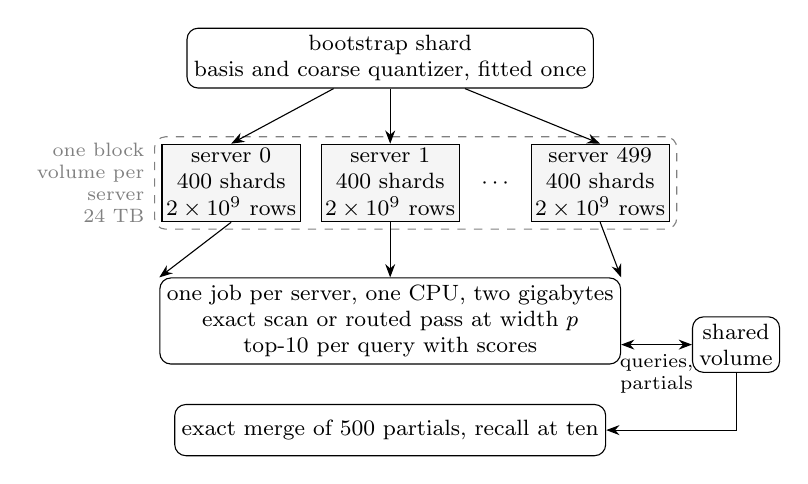
\begin{tikzpicture}[
  font=\footnotesize, node distance=4mm,
  box/.style={draw, rounded corners, align=center, minimum height=6.5mm, inner sep=2.5pt},
  srv/.style={draw, align=center, minimum width=13mm, minimum height=9mm, inner sep=1.5pt, fill=gray!8},
  >={Stealth[]}]
\node[srv] (s0) {server 0\\400 shards\\$2\times10^{9}$ rows};
\node[srv, right=2.5mm of s0] (s1) {server 1\\400 shards\\$2\times10^{9}$ rows};
\node[right=1.5mm of s1] (dots) {$\cdots$};
\node[srv, right=1.5mm of dots] (s499) {server 499\\400 shards\\$2\times10^{9}$ rows};
\node[box, above=7mm of s1] (boot) {bootstrap shard\\basis and coarse quantizer, fitted once};
\node[box, below=7mm of s1] (job) {one job per server, one CPU, two gigabytes\\exact scan or routed pass at width $p$\\top-10 per query with scores};
\node[box, right=9mm of job, yshift=-3mm] (shared) {shared\\volume};
\node[box, below=5mm of job] (merge) {exact merge of 500 partials, recall at ten};
\draw[->] (boot) -- (s0.north);
\draw[->] (boot) -- (s1.north);
\draw[->] (boot) -- (s499.north);
\draw[->] (s0.south) -- (job.north west);
\draw[->] (s1.south) -- (job.north);
\draw[->] (s499.south) -- (job.north east);
\draw[<->] (job.east |- shared.west) -- (shared.west) node[midway, below, font=\scriptsize, align=center]{queries,\\partials};
\draw[->] (shared.south) |- (merge.east);
\begin{scope}[on background layer]
\node[draw, dashed, gray, rounded corners, inner sep=2.5pt, fit=(s0)(s499), label={[gray, font=\scriptsize, align=right]left:one block\\volume per\\server\\24 TB}] {};
\end{scope}
\end{tikzpicture}
\caption{The fleet. One bootstrap shard fixes the projection basis and the 2048-cell coarse
quantizer for every shard on every server, so scores are comparable across servers and the
global top-10 is the exact merge of per-server top-10s. Each phase is one job per server, and
each job reads only its own volume and the shared volume.}
\label{fig:fleet}
\end{figure}

\paragraph{Index.} Each row is a 32-dimensional vector projected to 24 dimensions by one basis
shared by the whole fleet, quantized to 4 bits per dimension, and assigned to one of 2048
inverted-file cells by one shared coarse quantizer. Both the basis and the quantizer are fitted
once, on a bootstrap shard, and read by every build job. A shard holds five million rows. A
server holds 400 shards, two billion rows, on one block volume. The on-disk row is 12 bytes of
codes, 8 bytes of per-row norms used by the asymmetric distance computation, and 4 bytes of cell
membership. Every server reports 48\,009\,656\,624 index bytes for its two billion rows, 24.0
bytes per row, and the fleet holds 24.0 TB of index on 500 volumes. Scoring is asymmetric
distance computation over the codes, in row blocks, from memory-mapped shards. Because the basis
and the coarse quantizer are shared, scores from different shards are comparable and a global
top-$k$ is the exact merge of per-shard top-$k$s. That property is what makes an exact measurement
of the whole index possible, and Figure~\ref{fig:fleet} shows the arrangement.

\paragraph{Scale.} The same layout has been built and measured at $10^{8}$ rows on 4 servers,
$10^{9}$ on 4, $10^{10}$ on 8, $10^{11}$ on 50 and $10^{12}$ on 500. Per-server work is constant
from $10^{11}$ on, two billion rows, so the step from 50 to 500 servers changes nothing per node
and changes only the number of chances to draw a slow or failing one.

\section{The corpus is a seed, not a file}
\label{sec:corpus}

The corpus is defined by a seed and regenerated on demand. Each global shard draws a fresh
rank-16 Gaussian basis, projects Gaussian coefficients through it with a linear decay of singular
values from 1.0 to 0.3, and adds five percent noise, in an ambient dimension of 32. A shard is a
pure function of its global index, so any job can produce any shard without reading anything.
The companion paper \cite{bond2026recall} discusses what this corpus is and is not as a stand-in
for real embeddings. For the systems question it does three things.

It removes data movement. A build from files would first have to place the corpus, $10^{12}$
rows of 32 single-precision values, 128 TB, where 500 jobs could read it, and then read all of it
once. Built from a seed, each server's job computes its own 400 shards and writes only its share
of the 24 TB index. What moves is the code, its dependencies and the fitted bootstrap on the
shared volume, which every job reads, and the query cache and partial results, which are small.

It bounds memory. A build job streams its 400 shards from the seed in row bands, writes each
shard as it goes, and never holds a whole shard in memory. After each band it flushes the written
pages to the volume and tells the kernel to drop them, because the page cache of freshly written
data counts against the job's two-gigabyte limit and dirty pages cannot be reclaimed until they
are written. The job's own memory stays at a few hundred megabytes, one build pod measured 292 MiB
of anonymous memory beside 1526 MiB of file pages, and the build runs in the same one-CPU,
two-gigabyte class as the measurement.

It makes loss recoverable. The volumes are single-replica block volumes. Six of them became
unreachable when their node went offline. Each was deleted, recreated under the same name and
rebuilt from its seed, on the first attempt, in 2 hours 32 minutes to 3 hours 49 minutes. No
backup of the index was kept, because the seed and the code reproduce it.

\paragraph{Build.} The 500 servers were built between 2026-08-04 and 2026-09-24. The first 16
were built in waves and the remaining 484 by one pool with no wave barrier, the same pool the
measurement later used. Each server took between two and a half and four hours.

\section{Storage is one volume per server}
\label{sec:storage}

Each server's index lives on its own block volume of 56 GiB, mounted by exactly one job at a
time. Every job of a phase reads only its own volume and the shared network file system, so a
slow volume slows one server and no other. Volumes are
provisioned at a paced rate, because a burst of claims times out the provisioner. In August a new
volume bound in about 31 seconds, and the six replacements of September took about ten minutes.
Scans read the index through memory maps in blocks, so the page cache holds recently read index
pages. Those pages count against the job's memory limit, and the kernel reclaims them under it,
because they are clean copies of data on the volume.

\section{The measurement is a graph of idempotent phases}
\label{sec:phases}

\begin{table}[t]
\caption{The phases of the measurement. Every job writes its output under a temporary name and
renames it, and exits at once if the output exists, so any job can be re-run at any time. The
metadata phases read only partials and the index's cell metadata.}
\label{tab:phases}
\centering
\small
\setlength{\tabcolsep}{3pt}
\begin{tabular}{lrll}
\toprule
phase & jobs & reads & writes \\
\midrule
query cache    & 1   & seed & 100 queries \\
exact scan     & 500 & own volume, queries & top-10 per query \\
routed pass    & 500 & own volume, queries & top-10 per width \\
score          & 1   & 1500 partials & recall at ten \\
second sweep   & 500 & own volume, queries & top-10 at 16, 64, 256 \\
cell census    & 500 & own cell metadata & cell counts \\
census merge   & 1   & counts, partials & cell ranks \\
\bottomrule
\end{tabular}
\end{table}

Table~\ref{tab:phases} lists the phases. Each is a set of independent jobs, one per server or one
in all, and the driver runs the phases in order, so a phase that reads another's output starts
after it. Within a phase there is no order and no barrier, so a slow server delays only the
phase's last result. Every job reads its own volume and the shared volume and writes one small
file to the shared volume. The driver checkpoints each phase to a state file, and after a restart
it reloads that file and adopts the jobs still running on the cluster.

Idempotency is the property the rest of the design relies on. A job whose output exists prints
that fact and exits, and a job interrupted mid-write leaves only a temporary file that the next
attempt overwrites. A duplicate job, a retried job and a job the driver adopted after a restart
are therefore all harmless, and the recovery rules of Section~\ref{sec:pool} can re-issue a job
whenever its state is in doubt without risking a wrong or double-counted partial.

\section{Submissions yield to the cluster}
\label{sec:controller}

\begin{table}[t]
\caption{The submission controller's settings during the run and the pool's rules. The controller
decides when a submitted job is created. The pool decides when a job is re-issued.}
\label{tab:rules}
\centering
\small
\setlength{\tabcolsep}{3pt}
\begin{tabular}{@{}p{0.6\columnwidth}p{0.36\columnwidth}@{}}
\toprule
setting & value \\
\midrule
\multicolumn{2}{l}{\emph{controller}} \\
own running jobs at most & 20 \\
own pending jobs at most & 5 \\
cluster pending pods that trigger waiting & 100 \\
node CPU load that triggers waiting & 0.85 \\
wait before retrying a deferred job & 30 s, doubling to 15 min \\
attempts before giving up & 15 \\
\multicolumn{2}{l}{\emph{pool}} \\
jobs in flight at most & 20 \\
attempts per server & 40 \\
back-off after a failed job & 2 min, doubling to 30 min \\
wait for a submitted job to appear & 90 polls, one a minute \\
pending pod recycled after (first run) & 45 min \\
terminating pod removed after (second sweep) & 30 min \\
running job logged, not removed (second sweep) & 16 h \\
sweeps over parked servers & 12, 30 min apart \\
\bottomrule
\end{tabular}
\end{table}

Jobs are not created by the driver directly. The driver publishes each job to a controller
\cite{natsbursting} that runs beside it and decides when to create it. Before every creation the
controller looks at its own queue and at the cluster. It creates nothing while it already has five
of its own jobs pending or twenty running, and it waits while more than a hundred pods are pending
across the cluster or the target nodes are busy. A deferred job is retried after thirty seconds,
then after doubling waits up to fifteen minutes, for up to fifteen attempts. The scheme is the
carrier-sense and back-off rule of shared radio channels applied to a shared batch system, and it
follows an earlier design for polite submission to shared clusters \cite{politesubmit}. The effect
is that the run takes capacity when the cluster has it and gives way when other groups need it.

The pool above the controller has its own rules, listed in Table~\ref{tab:rules}. The one that
matters most is patience with the controller. A job the controller has deferred is not yet
visible to the cluster, and a driver that reads its absence as loss resubmits it and queues a
duplicate behind it. The pool therefore waits ninety minutes for a submitted job to appear before
it treats the job as lost.

\section{Every job fits one CPU and two gigabytes}
\label{sec:shape}

Every job in the measurement requests one CPU and two gigabytes of memory. That is the smallest
class the cluster offers, it is the class in which a fleet of hundreds of small jobs takes the
least from other users, and the sharded index needs nothing more once three choices are made in
how a scan over memory-mapped shards is written. The first is that the queries come from the
cache. Deriving the 100 queries from the seed means regenerating four whole five-million-row
blocks, about 640 MB each plus temporaries, so the query-cache phase writes the set once and every
scan reads the file. The second is that at most two shards are open. A memory-mapped shard still
materializes its row-id and tombstone arrays, 45 MB per five-million-row shard, and the sharded
index holds 128 shards open by default, 5.8 GB across a full scan. The scan holds two shards open
and the routed pass eight, with two worker threads. The third is that scoring proceeds in blocks
of 65536 rows, which bounds the per-block temporaries to tens of megabytes.

\begin{table}[t]
\caption{What one job of each kind used, in the one-CPU, two-gigabyte class. Memory is what the
job's control group is charged, which includes page cache. Own memory is the process's resident
set, or its anonymous memory for the build. The build row is one of the six servers rebuilt in
September. Cells the record does not hold are left empty.}
\label{tab:budget}
\centering
\footnotesize
\setlength{\tabcolsep}{2.5pt}
\begin{tabular}{lrrrrr}
\toprule
job & wall & mean cores & mean mem. & peak mem. & own mem. \\
\midrule
build          & 2.5--3.8 h &      &          & 2048 MiB & 292 MiB \\
exact scan     & 1912 s     & 0.88 & 1242 MiB & 1469 MiB & 346 MB \\
routed pass    & 36 min     & 0.48 & 1258 MiB & 1568 MiB & 165 MB \\
\bottomrule
\end{tabular}
\end{table}

Table~\ref{tab:budget} gives what one job of each kind used. The exact scan is compute-bound and
holds nearly one core. The routed pass reads less and computes less per byte, so it averages about
half a core. In both, most of the charged memory is page cache from the memory-mapped index, clean
pages that the kernel reclaims under the limit, and the processes themselves hold under 350 MB. A
routed pod was observed at the two-gigabyte limit with 224 MB anonymous and 1.9 GB of file pages,
and it completed normally. The build reaches the limit for the same reason, with written rather
than read pages, which is why it flushes and drops them band by band. The score job, which
merges 1500 small partials, and the metadata jobs, which read partials and cell metadata, run in
the same class in minutes and half a minute respectively.

\section{A pool of idempotent jobs carries the run}
\label{sec:pool}

\begin{figure}[t]
\centering
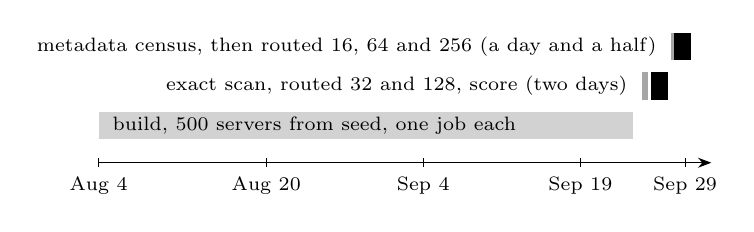
\begin{tikzpicture}[font=\scriptsize, >={Stealth[]}, x=0.133cm]
% x is days from 2026-08-04; the axis runs to 2026-09-30.
\draw[->] (0,0) -- (58.5,0);
\foreach \d/\l in {0/Aug 4, 16/Aug 20, 31/Sep 4, 46/Sep 19, 56/Sep 29} {
  \draw (\d,0.06) -- (\d,-0.06) node[below] {\l};
}
% build 2026-08-04 to 2026-09-24
\fill[gray!35] (0,0.3) rectangle (51,0.65);
\node[anchor=west] at (0.4,0.475) {build, 500 servers from seed, one job each};
% first run: 09-24 20:41 to 09-25 10:10 at the earlier job shape, then 09-25 18:01 to 09-27 08:59
\fill[gray!70] (51.86,0.8) rectangle (52.42,1.15);
\fill[black] (52.75,0.8) rectangle (54.37,1.15);
\node[anchor=east] at (51.4,0.975) {exact scan, routed 32 and 128, score (two days)};
% census 09-27 16:32 to 21:29, then routed 16, 64 and 256 from 09-27 21:37 to 09-29 12:56
\fill[gray!70] (54.69,1.3) rectangle (54.9,1.65);
\fill[black] (54.9,1.3) rectangle (56.54,1.65);
\node[anchor=east] at (54.2,1.475) {metadata census, then routed 16, 64 and 256 (a day and a half)};
\end{tikzpicture}
\caption{The run on the calendar. The index was built over seven weeks by a pool of one job
per server. The measurement, the census and the second sweep took four days at the end of
September, all through the same controller.}
\label{fig:timeline}
\end{figure}

\begin{figure}[t]
\centering
\begin{tikzpicture}
\begin{axis}[
  width=0.95\columnwidth, height=4.2cm,
  xmin=0, xmax=40, ymin=0, ymax=23,
  xlabel={hours since the start of the run},
  ylabel={jobs in flight},
  ytick={0,5,10,15,20},
  grid=major, grid style={gray!25},
  legend pos=south west, legend style={font=\scriptsize, draw=none, fill=white, fill opacity=0.8, text opacity=1},
  tick label style={font=\footnotesize}, label style={font=\footnotesize},
]
\addplot[color=black, thick, const plot] table[x=hours, y=inflight] {../pvldb1t/figdata/inflight_first_run.dat};
\addlegendentry{first run}
\addplot[color=black!45, thick, const plot, dashed] table[x=hours, y=inflight] {../pvldb1t/figdata/inflight_second_sweep.dat};
\addlegendentry{second sweep}
\end{axis}
\end{tikzpicture}
\caption{Jobs the pool had in flight, from the driver logs, for the first run (exact scan, routed
passes at 32 and 128 probes, score) and the second sweep (routed passes at 16, 64 and 256
probes, score). The pool holds the controller's cap of twenty until each phase drains.}
\label{fig:inflight}
\end{figure}

The measurement was driven by a pool of at most twenty jobs in flight with no wave barrier,
checkpointed per phase, restartable, and able to adopt jobs already on the cluster after a
restart. Figure~\ref{fig:timeline} places it on the calendar, Figure~\ref{fig:inflight} shows how
full the pool stayed, and Table~\ref{tab:pool} gives what it did. The median number of jobs in
flight was nineteen in both runs. The first run finished 835 jobs that it ran itself in 39 hours,
and found 14 more whose output already existed, and the second sweep finished 501 in 39 hours.
The rules come first because the counts are only meaningful against them.

\begin{table}[t]
\caption{The pool over the first run, 2026-09-25 18:01 UTC to 2026-09-27 08:59 UTC, and the
second sweep, 2026-09-27 21:37 UTC to 2026-09-29 12:56 UTC. First-run scan counts exclude 152
servers scanned in an earlier session at a larger job shape.}
\label{tab:pool}
\centering
\small
\begin{tabular}{lrr}
\toprule
 & first run & second sweep \\
\midrule
submissions & 928 & 574 \\
completions & 849 & 501 \\
recycles after a failed job & 75 & 73 \\
\quad storage read fault on one node & 24 & 25 \\
\quad node lost during the job & 13 & 17 \\
\quad node unreachable, pod stuck & 13 & 11 \\
\quad container start failure & 2 & 1 \\
\quad other & 23 & 19 \\
recycles after 45 minutes pending & 26 & 0 \\
submissions deferred by the controller & 1 & 0 \\
servers parked or given up & 0 & 0 \\
\bottomrule
\end{tabular}
\end{table}

\paragraph{Rules.} A job whose Kubernetes object reports success is done. A job whose object
reports failure is recycled, meaning its object is deleted and, after an exponential back-off from
two minutes to thirty, resubmitted, up to forty times before the server is parked and swept again
later. A job submitted through the controller but not yet visible as an object is waited on for
ninety polls, one a minute, before it is treated as lost. In the first run a job whose pod had not
reached the running state 45 minutes after submission was recycled the same way. For the second
sweep that rule was replaced by waiting, because a running job is never deleted on a namespace
other groups share, and a job running longer than sixteen hours is logged rather than removed.

\paragraph{The deferral rule.} The submission controller defers creating a job while the
namespace already has several pending or the cluster is busy, and retries for up to about an
hour. A driver that treats a deferred submission as a lost one resubmits, and every resubmission
queues a duplicate behind the original it was meant to replace. The wait before a submission is
treated as lost separates the two cases. The run needed the rule once, for the score job.

\paragraph{Failure classes.} Two dominated, and both are ordinary on a shared cluster. One node
returned a storage read fault to every job placed on it within 3 to 13 minutes of start,
after its block volume had attached. Retries landed elsewhere and finished, at a cost of about 130
slot-minutes out of 9600 over the first eight hours. The second class, pods pending past 45
minutes, was benign in every instance checked, because the original pod had run and the retry
found its output within minutes. That is what idempotent jobs buy. In the second sweep 63 servers
needed a second attempt, 9 a third and 1 a fourth, and a storage fault at one moment ended all
twenty jobs in flight at once, after which fresh submissions ran and the batch was re-issued after
its back-off.

\paragraph{Pods that stop answering.} A pod can stay in a terminating state on a node that
no longer responds, or run on a node whose storage path is slow, and the job controller does
not replace it on its own. Four such pods in the first run and two in the second sweep were
removed by hand, and their replacements finished normally. The second sweep added a rule
for pods terminating longer than thirty minutes. Across four days the manual actions were six
pod removals and one resubmission of the score job.

\paragraph{Provenance.} The job containers cloned the repository's default branch at run time,
and twelve commits appear in pod logs across the first run. The phase scripts came from a
configuration map fixed for each run, and the merge and score code did not change. Pinning the
clone to a commit is the one change to the descriptor for the next run.

\section{The measurement cost 1349 CPU-hours}
\label{sec:cost}

\begin{table}[t]
\caption{Per-server wall time in the $10^{12}$ run, one CPU per job, 500 servers per phase, and
the CPU-hours each phase consumed. The three routed widths of the second sweep ran inside one
job per server and share its start-up. Each time includes pulling the image, installing
dependencies, cloning the repository and opening 400 shards from network block storage, so it is
the cost of the measurement job and not of inverted-file search. Derived from the record by
\texttt{paper/pvldb1t/figdata/fig\_data.py}.}
\label{tab:cost}
\centering
\small
\begin{tabular}{lrrrrrr}
\toprule
phase & median & mean & p10 & p90 & max & CPU-h \\
\midrule
exact scan       & 2664 s & 3008 s & 1850 s & 4009 s & 16308 s & 418 \\
routed, 32       & 1064 s & 1131 s &  775 s & 1466 s & 14286 s & 157 \\
routed, 128      & 1335 s & 1420 s &  958 s & 1861 s & 14524 s & 197 \\
routed, 16       &  916 s & 1071 s &  660 s & 1440 s & 12236 s & 149 \\
routed, 64       & 1219 s & 1366 s &  912 s & 1743 s & 14645 s & 190 \\
routed, 256      & 1594 s & 1719 s & 1176 s & 2199 s & 13786 s & 239 \\
\bottomrule
\end{tabular}
\end{table}

\begin{figure}[t]
\centering
\begin{tikzpicture}
\begin{axis}[
  width=0.95\columnwidth, height=5cm,
  xmode=log, log basis x=10,
  xmin=300, xmax=20000,
  ymin=0, ymax=1.02,
  xlabel={per-server wall time (s)},
  ylabel={share of servers at or below},
  xtick={300,1000,3000,10000},
  xticklabels={300,1000,3000,10000},
  ytick={0,0.25,0.5,0.75,1},
  grid=major, grid style={gray!25},
  legend pos=south east, legend style={font=\scriptsize, draw=none, fill=none},
  legend cell align=left,
  tick label style={font=\footnotesize}, label style={font=\footnotesize},
]
\addplot[color=black, thick] table {../pvldb1t/figdata/ecdf_exact_scan.dat};
\addlegendentry{exact scan}
\addplot[color=black!75, thick, dashed] table {../pvldb1t/figdata/ecdf_routed_256.dat};
\addlegendentry{routed, 256}
\addplot[color=black!65, thick, dotted] table {../pvldb1t/figdata/ecdf_routed_128.dat};
\addlegendentry{routed, 128}
\addplot[color=black!55, thick, dashdotted] table {../pvldb1t/figdata/ecdf_routed_64.dat};
\addlegendentry{routed, 64}
\addplot[color=black!45, thick, densely dashed] table {../pvldb1t/figdata/ecdf_routed_32.dat};
\addlegendentry{routed, 32}
\addplot[color=black!35, thick, densely dotted] table {../pvldb1t/figdata/ecdf_routed_16.dat};
\addlegendentry{routed, 16}
\end{axis}
\end{tikzpicture}
\caption{Distribution of per-server wall time by phase, 500 servers each, one CPU per job. The
bodies are tight and the tails are a few servers on slow nodes, which the pool absorbs by
waiting rather than by re-placing. Data derived from the record logs.}
\label{fig:wall}
\end{figure}

Table~\ref{tab:cost} and Figure~\ref{fig:wall} give what the measurement cost. The exact scan
of two billion rows at one CPU takes 44 minutes at the median and the routed pass 15 to 27
minutes depending on width. The first run, exact scan and routed passes at 32 and 128, consumed
772 CPU-hours, and the second sweep at 16, 64 and 256 consumed 577, so the whole measurement is
1349 CPU-hours of the cluster's smallest job class. The routed times are not the cost of inverted-file search, and the ratio between the routed and
exact rows is not a latency figure for the method. These jobs are read-bound on network block storage,
spend a fixed minute or two on image pull, dependency install and clone, and open 400 shards
before scoring. The $10^{11}$ run, on six CPUs per job, reported 14.7 and 8.5 as the same ratio,
and neither number is the method's. The tails are node variance. Between 4 and 30 servers per
phase took more than twice the median, the 16308 s maximum of the scan is one server on one
node that also produced the slowest routed pass, and in every phase the ninetieth percentile is
within 1.6 times the median.


\section{Seven design choices, each against its obvious alternative}
\label{sec:lessons}

Table~\ref{tab:design} collects the choices. Each one replaces a choice that is reasonable at a
billion rows with one that stays reasonable at a trillion, and each is measured in the run rather
than argued. None depends on vector search. A seeded generator, bounded jobs that are safe to
repeat, and a pool that waits for the platform instead of racing it apply to any computation that
is too large for one machine and too small to justify reserved capacity.

We would change three things. The job containers cloned the repository's default branch at run
time, so the code that ran moved as the branch moved, and the next run pins the clone to one
commit. A rule for pods that stay in a terminating state now exists in the driver, and the next
run starts with it. The query set came from four seeded shards, which concentrates the reference
neighbours on few servers, and the companion paper measures a query set drawn from seeds no
corpus shard uses.
% NONMEMBER-QUERIES PENDING: keep this sentence only if the companion paper carries the 1tnm result.

\section{Related work}

Distributed vector databases such as Milvus \cite{wang2021milvus} and its cloud-native successor
\cite{guo2022manu} shard an index across nodes and merge per-node results, which is the arrangement
our fleet uses without a serving layer. Billion-scale practice with Faiss
\cite{johnson2019faiss,douze2024faiss}, DiskANN \cite{subramanya2019diskann} and SPANN
\cite{chen2021spann} places an index on one machine or one node's disk, and the Big ANN
competitions \cite{simhadri2022bigann,simhadri2024bigann23} fixed datasets and reporting at
$10^{9}$ rows. Recent work places a billion-scale index on distributed storage \cite{yu2025dsann}.
The National Research Platform \cite{weitzel2025nrp} describes the federated cluster this run used.
We found no published account of building and exactly scanning a $10^{12}$-row vector index on a
shared cluster in its smallest job class.

\section{Reproducibility}

The repository at the availability URL carries the corpus seeds and generator, the build, scan,
routed, score and metadata scripts, the pool driver with its rules, and, under the directory
\texttt{benchmarks/fleet/} \texttt{record/1t/}, the pool state files, every driver log, the pilot logs and the
score logs whose RESULT\_JSON lines hold every per-server wall time. The cost table and the
wall-time figure are produced from those logs by \texttt{paper/pvldb1t/figdata/}
\texttt{fig\_data.py}.
Rebuilding the index from seed costs about three and a half hours per server at the pool's width.

\section{Conclusion}

A trillion-row vector index was built from a seed and measured exactly on a shared research
cluster in the smallest job class it offers. The build moved no corpus bytes, a lost volume was a
four-hour rebuild, and a pool of idempotent jobs with explicit rules for failure, waiting and
deferral carried the four-day measurement, 1349 CPU-hours, through the failures a shared cluster
produces, with six pods replaced by hand.

\begin{acks}
This work used the National Research Platform's Nautilus cluster. The National Research Platform
is supported in part by National Science Foundation awards CNS-1730158, ACI-1540112, ACI-1541349,
OAC-1826967, OAC-2112167, CNS-2100237 and CNS-2120019. We thank its operators and community.
\end{acks}

\bibliographystyle{ACM-Reference-Format}
\bibliography{refs}

\end{document}
